\section{Ejercicio 5}


\subsection{Desarrollo}
En el ejercicio se pide diseñar un lote con tres tareas de 50 ciclos y dos de 5 llamadas bloqueantes de 3 ciclos de duración. El lote que representamos inicia todas las tareas a la vez
\begin{verbatim}
TaskCPU 50
TaskCPU 50
TaskCPU 50
TaskConsola 5 3 3
TaskConsola 5 3 3
\end{verbatim}
Se pide calcular latencia, waiting time y tiempo total de ejecución 
\subsection{Experimentación}
\begin{figure}[H]
  \centering
    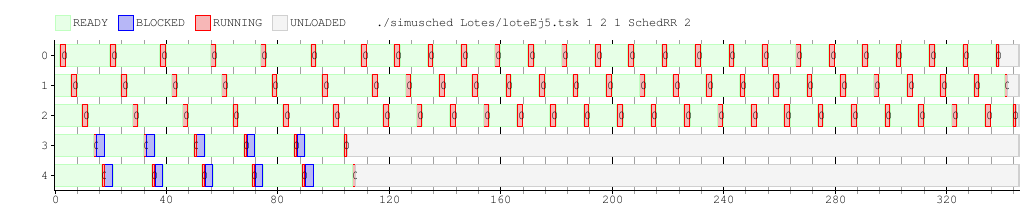
\includegraphics[width=1.1\textwidth]{imagenes/Ej5_q2.png}
  \caption{loteEj5.tsk con RR y quantum 2}
\end{figure}
\begin{figure}[H]
  \centering
    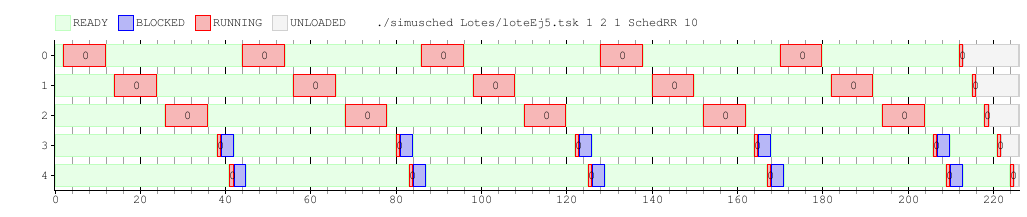
\includegraphics[width=1.1\textwidth]{imagenes/Ej5_q10.png}
  \caption{loteEj5.tsk con RR y quantum 10}
\end{figure}
\begin{figure}[H]
  \centering
    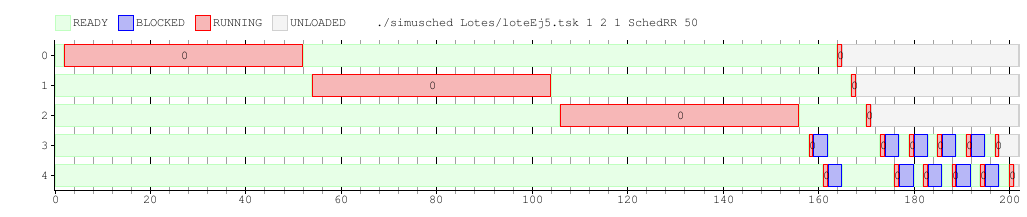
\includegraphics[width=1.1\textwidth]{imagenes/Ej5_q50.png}
  \caption{loteEj5.tsk con RR y quantum 50}
\end{figure}
\paragraph{quantum: 2}\par
\begin{tabular}{ l | c | c | c | c | c | c | }
  \hline			
  pid & ciclos & inicio & fin & latencia & waiting time & tiempo total  \\
  \hline
 0 & 51 & 0 & 339 & 2 & 288 & 339\\
1 & 51 & 0 & 342 & 6 & 291 & 342\\
2 & 51 & 0 & 345 & 10 & 294 & 345\\
3 & 21 & 0 & 105 & 14 & 84 & 105\\
4 & 21 & 0 & 108 & 17 & 87 & 108\\
  \hline
\end{tabular}
\paragraph{quantum: 10}\par
\begin{tabular}{ l | c | c | c | c | c | c | }
  \hline			
  pid & ciclos & inicio & fin & latencia & waiting time & tiempo total  \\
  \hline
0 & 51 & 0 & 213 & 2 & 162 & 213\\
1 & 51 & 0 & 216 & 14 & 165 & 216\\
2 & 51 & 0 & 219 & 26 & 168 & 219\\
3 & 21 & 0 & 222 & 38 & 201 & 222\\
4 & 21 & 0 & 225 & 41 & 204 & 225\\
\hline
\end{tabular}
\paragraph{quantum: 50}
\begin{tabular}{ l | c | c | c | c | c | c | }
  \hline			
  pid & ciclos & inicio & fin & latencia & waiting time & tiempo total  \\
  \hline
0 & 51 & 0 & 165 & 2 & 114 & 165\\
1 & 51 & 0 & 168 & 54 & 117 & 168\\
2 & 51 & 0 & 171 & 106 & 120 & 171\\
3 & 21 & 0 & 198 & 158 & 177 & 198\\
4 & 21 & 0 & 201 & 161 & 180 & 201\\
  \hline
\end{tabular}
